\section{Требования к системе}

\subsection{Функциональные требования}

\subsubsection{Диаграммы Вариантов Использования}

Функциональные требования заданы для ролей обзора системы. На диаграмме они собраны в четырёх акторах.

\begin{itemize}
\item \textbf{Клиент}~--- представитель юридического лица.
\item \textbf{Сотрудник}~--- клиентский менеджер, кредитный аналитик, андеррайтер и специалист финансового мониторинга.
\item \textbf{Администратор}~--- администратор правил хранения, руководитель и администратор системы.
\item \textbf{Внешние системы}~--- источники обязательных проверок, кредитной истории, налоговой и судебной информации.
\end{itemize}

Диаграмма приведена на рисунке~\ref{fig:usecase}. Система обеспечивает следующую функциональность:

\begin{itemize}
\item подать сведения об организации, лицах и долях (представитель);
\item вести заявку и выбрать кредитные условия (клиентский менеджер);
\item посмотреть результат, срок действия и причину отказа по своей заявке (представитель);
\item начать проверку (клиентский менеджер);
\item идентифицировать организацию и лиц, провести обязательные проверки, учесть показатели и запросить внешние сведения (сотрудник, внешние системы);
\item оформить корпоративное одобрение и обеспечение, когда сделка этого требует (клиентский менеджер);
\item вынести заключение (андеррайтер);
\item вести участие и владение (специалист финансового мониторинга);
\item задавать правила хранения (администратор правил хранения);
\item читать отчёты по заявкам, отказам и уровню риска (руководитель);
\item заводить сотрудников и назначать роли (администратор системы).
\end{itemize}

\begin{figure}[p]
\centering
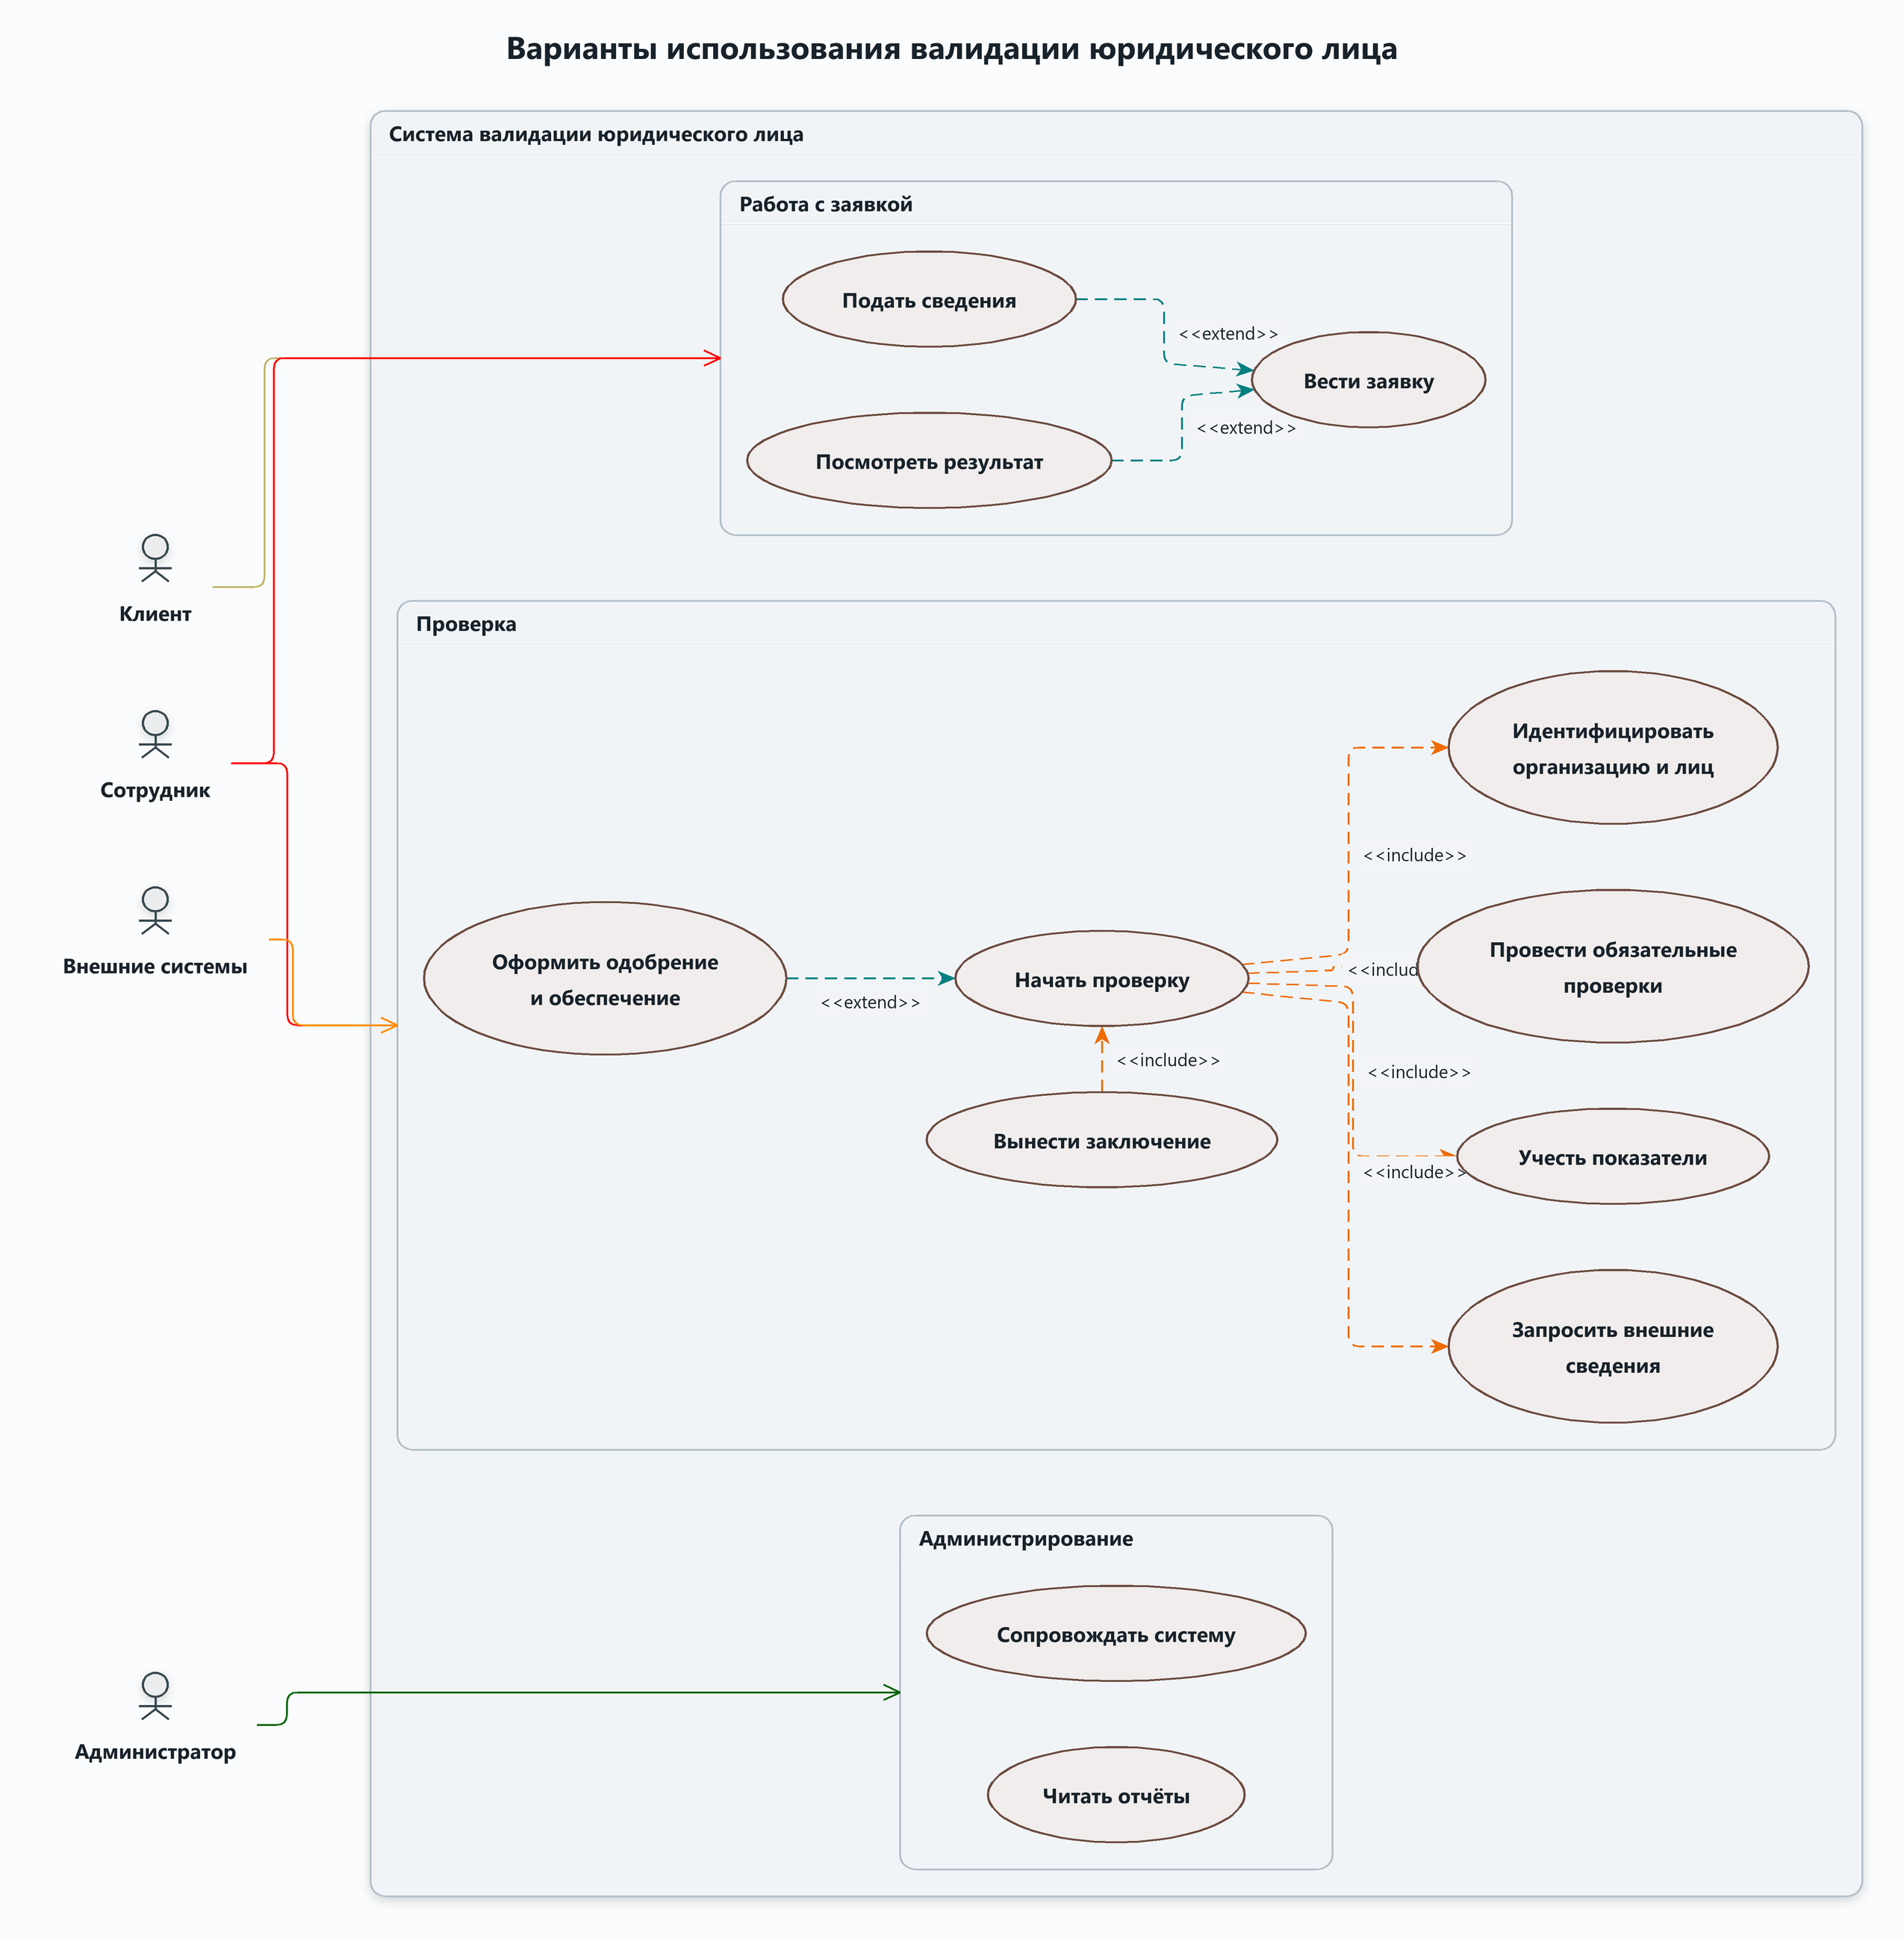
\includegraphics[width=\textwidth]{use_case_validaciya.png}
\caption{Диаграмма вариантов использования системы валидации юридического лица}
\label{fig:usecase}
\end{figure}

<<Подать сведения>> и <<Посмотреть результат>> расширяют вариант <<Вести заявку>>. <<Начать проверку>> включает идентификацию, обязательные проверки, учёт показателей и запрос внешних сведений. <<Оформить одобрение и обеспечение>> расширяет проверку: этих записей может не быть. <<Вынести заключение>> включает <<Начать проверку>>.

\subsubsection{Спецификация ключевых Вариантов Использования}

\textbf{Ведение заявки.}

Акторы: представитель юридического лица, клиентский менеджер.

Основной сценарий: представитель передаёт сведения об организации, лицах и долях. Менеджер создаёт заявку, указывает сумму, срок, валюту, канал и цель проверки и выбирает одни кредитные условия. Повторная проверка создаёт новую заявку.

Результат: заявка ссылается ровно на одни кредитные условия.

\textbf{Начало проверки.}

Акторы: клиентский менеджер, внешние системы.

Основной сценарий: менеджер отправляет заявку на проверку. Система идентифицирует организацию и участие, при длинной цепочке читает владение, проверяет действующее согласие и записывает обязательные проверки с нормой, источником и датой. Внешние сведения запрашиваются, когда проверка использует персональные данные или кредитную историю. Заявка на проверке без обязательной проверки не принимается.

Результат: у заявки есть одна или несколько обязательных проверок.

\textbf{Учёт показателей.}

Акторы: кредитный аналитик.

Основной сценарий: аналитик вносит финансовую отчётность и показатели. Показатель без отчёта допустим, если источник~--- суд, налог или бюро. В заявку показатель попадает связью <<Учтено>>: вес, порог и вывод. Вывод~--- усиливает, ослабляет или блокирует. Новая редакция условий не меняет уже записанный вес.

Результат: у заявки зафиксированы учтённые показатели с выводом по её условиям.

\textbf{Вынесение заключения.}

Акторы: андеррайтер.

Основной сценарий: андеррайтер читает проверки, учтённые показатели, условия, одобрение и обеспечение. Непройденная обязательная проверка или вывод <<блокирует>> закрывают положительный результат. Заключение получает результат, уровень риска, срок действия и, при отказе, причину. Пересмотр добавляет новое заключение и сохраняет предыдущее.

Результат: у заявки есть заключение. Офис и интернет-банк получают один уровень риска при тех же организации, показателях и условиях.

\textbf{Ведение цепочки владения.}

Акторы: специалист финансового мониторинга.

Основной сценарий: специалист записывает участие и владение: долю, основание, руководителя и бенефициара. Косвенная доля считается произведением долей по цепочке. Бенефициарный владелец~--- физическое лицо.

Результат: цепочка организаций и участия сохранены вместе с клиентом.

\textbf{Отчёты и сопровождение.}

Акторы: руководитель, администратор правил хранения, администратор системы.

Основной сценарий: руководитель читает отчёты по заявкам, отказам и уровню риска. Администратор правил задаёт категорию, основание, срок и событие начала отсчёта. Администратор системы заводит сотрудников и назначает роли.

Результат: правила хранения и роли заданы, отчёт сформирован.

\subsubsection{Дополнительные функциональные требования}

\begin{itemize}
\item поиск организации и заявки по ИНН, ОГРН, наименованию и номеру заявки;
\item запрос кредитной истории и иных внешних сведений только при действующем согласии;
\item выгрузка отчёта руководителя в PDF;
\item журнал действий сотрудников со сроком хранения пять лет;
\item неотправленный черновик заявки живёт один год и в пакет заявки не входит.
\end{itemize}

\subsection{Требования к экранным формам}

\begin{itemize}
\item \textbf{Форма входа.} Логин, пароль и роль. Дальше открываются только разделы этой роли.
\item \textbf{Главное меню.} Организация, заявки, проверки, отчёты, правила хранения. Состав пунктов зависит от роли.
\item \textbf{Карточка организации.} Наименование и организационно-правовая форма, ИНН, ОГРН и ОКВЭД, статус, адрес, лицензия, участия, владение и согласия.
\item \textbf{Форма заявки.} Номер, дата и канал, сумма, срок и валюта, статус и цель, выбранные кредитные условия, проверки, связь <<Учтено>>, одобрение, обеспечение и заключения.
\item \textbf{Форма заключения.} Результат проверки, уровень риска, срок действия и причина отказа. Представитель видит по своей заявке результат, срок и причину отказа.
\item \textbf{Форма отчётов и правил хранения.} Период, статус и уровень риска. Отдельно~--- категория сведений, основание, срок и событие начала отсчёта.
\end{itemize}

\subsection{Нефункциональные требования}

\textbf{Производительность.} Система обеспечивает одновременную работу сотрудников офиса и представителей в интернет-банке: не менее 200 сеансов. Время отклика при чтении карточки и заявки не превышает 2 секунд, при записи заявки, проверки и заключения~--- 3 секунд.

\textbf{Надёжность.} База защищает данные при сбое и восстанавливается из резервной копии до последнего согласованного состояния. Заявка, проверки, записи <<Учтено>> и заключение фиксируются одной транзакцией. Снятие пакета не удаляет клиента, показатель и редакцию условий.

\textbf{Безопасность.} Доступ разделён по ролям обзора. Представитель читает только свою заявку. Пароли хранятся в хешированном виде. Персональные данные и кредитная история обрабатываются при действующем согласии и по требованиям законодательства о персональных данных и о противодействии отмыванию доходов.

\textbf{Масштабируемость.} Новая редакция кредитных условий, новый вид обязательной проверки и новый канал подачи добавляются без смены уже накопленных заявок. Четыре категории хранения сохраняют свои сроки.
